\section{Estrutura bibliométrica do campo}
\label{sec:bibliometriaampliada}

A camada bibliométrica utilizou 372 registros com aderência simultânea ao objeto predial, à manutenção ou gestão, à sustentabilidade e à presença de método, dados ou resultados. Desse conjunto, 109 também integram o núcleo temático vigente, 263 são exclusivos da camada bibliométrica e 12 pertencem apenas ao núcleo temático; as duas camadas cumprem, portanto, funções analíticas complementares. Todos os registros possuíam título, ano, fonte e resumo; 329 (88,4\%) continham palavras-chave, 327 (87,9\%) DOI e 91 (24,5\%) autores. A completude disponível sustentou as análises de fontes e palavras-chave, enquanto afiliações e referências citadas seriam necessárias para redes representativas de colaboração e acoplamento.

As palavras-chave foram normalizadas quanto a caixa, acentuação, singular e variantes ortográficas, reunindo, por exemplo, \textit{building information modeling}, \textit{building information modelling} e BIM. A rede considera coocorrência no mesmo registro normalizada pelo cosseno das frequências marginais; o mapa temático posiciona os 40 termos mais frequentes por centralidade externa e densidade interna; e a evolução compara 157 registros de 2010--2020 com 215 de 2021--2026. Essas medidas descrevem associações documentais, com interpretação restrita à estrutura temática do corpus.

O Gráfico~\ref{fig:fontes372} sintetiza 208 fontes. O núcleo aproximado de Bradford reuniu 13 delas, responsáveis por cerca de um terço dos registros. \textit{Energy and Buildings} apresentou 18 registros, seguida por \textit{Journal of Building Engineering} (15), \textit{Facilities} (14), \textit{Lecture Notes in Civil Engineering} (11), \textit{IOP Conference Series: Earth and Environmental Science} (10) e \textit{Sustainability} (10). A combinação de energia, engenharia de edificações, gestão de facilidades e sustentabilidade confirma a natureza interdisciplinar do campo.

\begin{figure}[htbp]
\centering
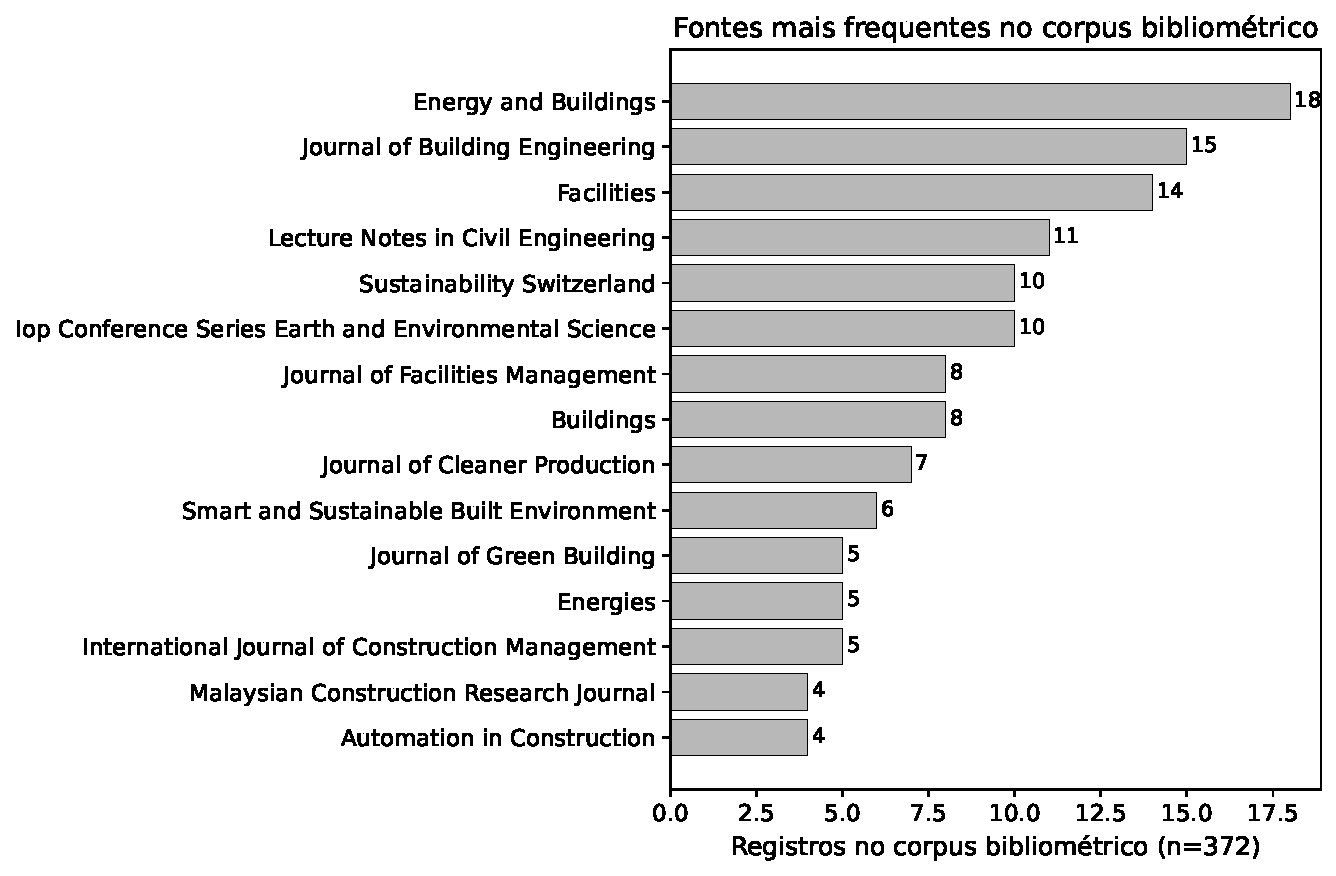
\includegraphics[width=0.98\linewidth]{figuras/figura_fontes_relevantes_372.pdf}
\captiongrafico{Fontes mais frequentes no corpus bibliométrico ampliado}
\label{fig:fontes372}
\end{figure}

O mapa temático (Gráfico~\ref{fig:mapatematico372}) revelou dois eixos centrais. O primeiro articulou BIM, desempenho da edificação e \textit{digital twins}, com centralidade e densidade acima das medianas; o segundo aproximou gestão de facilidades, edifícios inteligentes e manutenção preditiva, com elevada centralidade e menor densidade interna. Edificações verdes, avaliação do ciclo de vida e desenvolvimento sustentável formaram grupos mais especializados, enquanto energia, emissões e operação predial permaneceram semanticamente heterogêneas.

\begin{figure}[htbp]
\centering
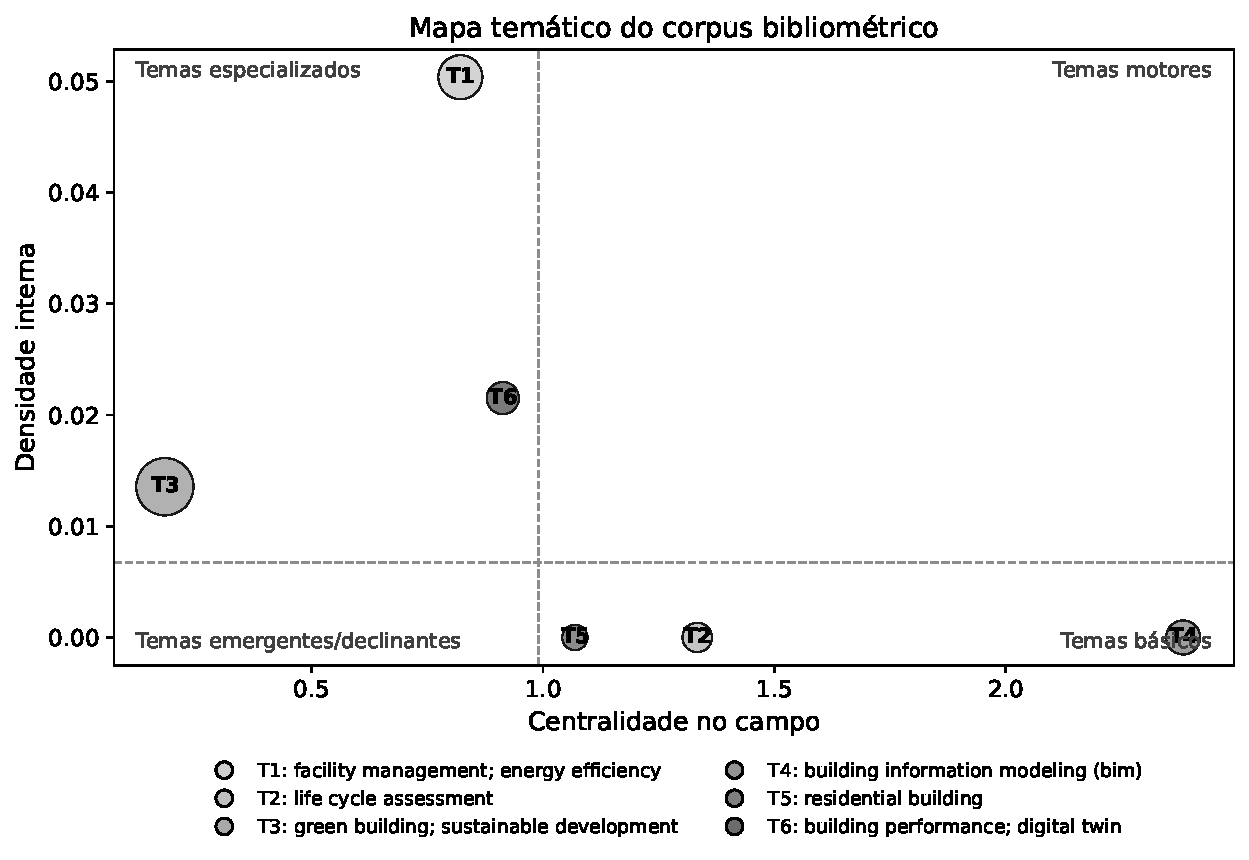
\includegraphics[width=0.98\linewidth]{figuras/figura_mapa_tematico_372.pdf}
\captiongrafico{Mapa temático por centralidade e densidade das palavras-chave}
\label{fig:mapatematico372}
\end{figure}

A rede normalizada (Gráfico~\ref{fig:redecor372}) reforça BIM e gestão de facilidades como conectores. BIM associa-se a gestão de facilidades, \textit{digital twins}, manutenção preditiva, operação e desempenho; gestão de facilidades, a desempenho, operação e manutenção, gestão de ativos e internet das coisas. Em outro agrupamento, avaliação do ciclo de vida aproxima-se de edificações residenciais e desenvolvimento sustentável. As ligações registram vocabulários compartilhados e orientam a síntese temática subsequente.

\begin{figure}[htbp]
\centering
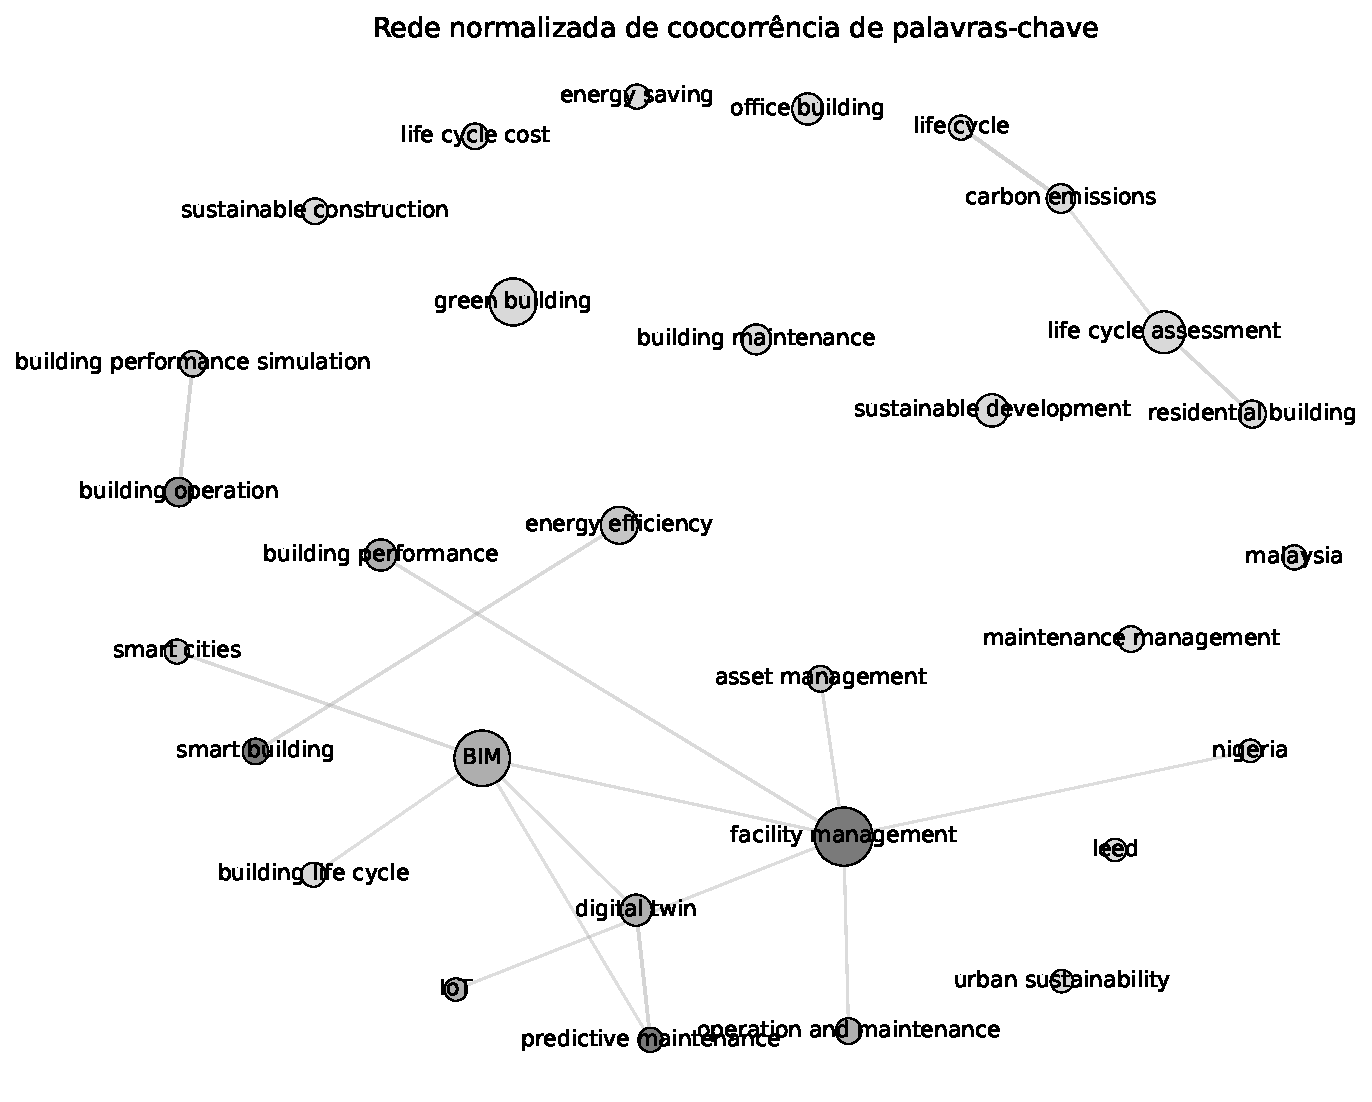
\includegraphics[width=0.98\linewidth]{figuras/figura_rede_coocorrencia_372.pdf}
\captiongrafico{Rede normalizada de coocorrência de palavras-chave}
\label{fig:redecor372}
\end{figure}

A comparação temporal (Gráfico~\ref{fig:evolucaotematica372}) mostrou aumento de 7,3 pontos percentuais para BIM, 4,7 para \textit{digital twins}, 2,7 para emissões de carbono e 1,9 para avaliação do ciclo de vida. Edificação verde, eficiência energética, manutenção predial e desempenho da edificação perderam participação relativa, movimento compatível com a incorporação de temas tradicionais a vocabulários tecnológicos e de ciclo de vida mais específicos.

\begin{figure}[htbp]
\centering
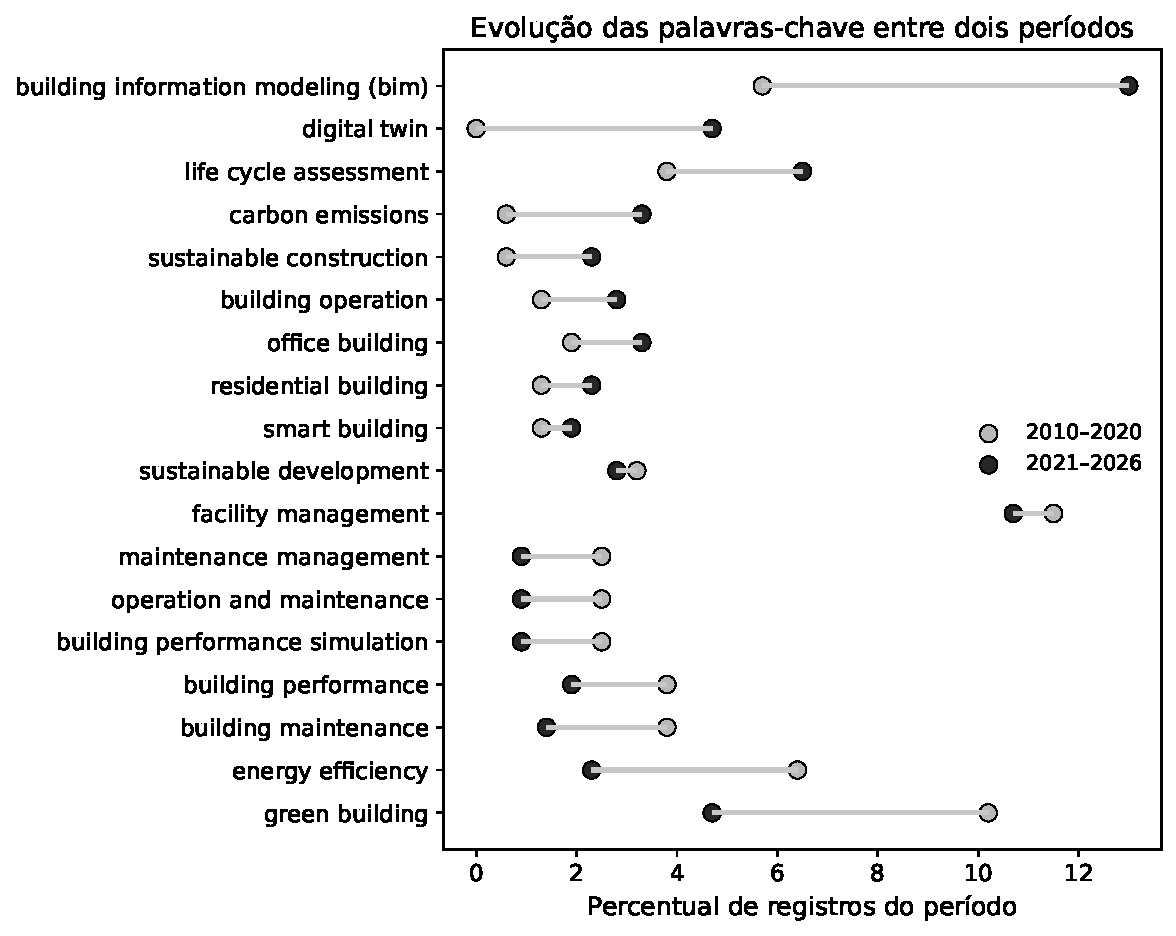
\includegraphics[width=0.98\linewidth]{figuras/figura_evolucao_tematica_372.pdf}
\captiongrafico{Evolução das palavras-chave entre 2010--2020 e 2021--2026}
\label{fig:evolucaotematica372}
\end{figure}

Em conjunto, a bibliometria indica transição de eficiência, desempenho e edificações verdes para BIM, \textit{digital twins}, carbono, ciclo de vida e manutenção preditiva. A síntese dos 121 registros, apresentada a seguir, verifica como essa transição se converte em dimensões, critérios, métodos e regras aplicáveis à priorização pública universitária.